\documentclass[../../../main.tex]{subfiles}
\graphicspath{{sections/part2/images/}}
\begin{document}
Probablement la section la plus simple de ce document, l'utilisation des pointeurs n'induira jamais de bogues étranges et inexpliqués dans un programme C. Tout un chacun peut affirmer sans hésitation qu'il n'y a rien de plus \textit{trivial} que la programmation avec des pointeurs.\newline
Tout va bien se passer\dots\newline
Maintenant que le lecteur est \textbf{\underline{\textit{rassuré}}}, commençons\dots
 
\textbf{Rappel :} Une variable peut être approximée comme la collection de trois informations :
\begin{itemize}
	\item une étiquette, aussi appelée le nom de de la variable
	\item une adresse mémoire
	\item une donnée sur $N$ octets à cette adresse
\end{itemize}
Visuellement : 

\begin{minipage}{\textwidth}
	\begin{center}
		\includesvg[width=.25\textwidth]{variable}
	\end{center}
\end{minipage} 

L'idée des pointeurs est simple : au lieu de stocker directement une valeur, on stocke l'adresse mémoire d'une autre variable :
 
\begin{minipage}{\textwidth}
	\begin{center}
		\includesvg[width=.4\textwidth]{pointeur}
	\end{center}
\end{minipage}
 
Les pointeurs sont fondamentaux en programmation. En particulier, ils permettent une flexibilité très importante des programmes écrits. La raison est simple : une variable est définie dans un certain espace. Ainsi, une variable d'une routine est locale à cette routine, et n'existe pas en dehors. Une adresse mémoire peut potentiellement exister hors de routines spécifiques. Cela amène cependant un inconvénient : en perdant un contrôle absolu sur l'existence de données, il devient possible \textit{par erreur} d'accéder à des zones mémoires qui ne sont plus utilisés. Il s'agit là de l'erreur la plus classique en programmation en C\footnote{traduite par le fameux message d'erreur \textit{Segmentation Fault}}.
 
On dispose pour la manipulation des pointeurs de deux opérateurs en langage C : l'étoile $\ast$ et l'esperluette $\&$. On a également la constante \textsf{NULL} qui représente un pointeur ne pointant sur rien du tout. 
Un pointeur est définit selon la syntaxe suivante :
\begin{minted}[linenos=false]{c}
TYPE* ptr;
\end{minted}
On sait alors que $ptr$ contiendra l'adresse d'autres variables.
 
Viens alors l'utilisation de l'esperluette. Ce caractère en tant qu'opérateur binaire permet de signifier l'opération $ET$, qu'elle soit logique ou bit-à-bit. Il est cependant possible de l'utiliser comme opérateur unaire. Sa signification est alors tout autre. \textsf{\&v} renvoie l'adresse mémoire à laquelle se situe la variable \textsf{v}. On peut donc écrire :
\begin{minted}[linenos=false]{c}
TYPE v = ...;
TYPE* ptr = &v;
\end{minted}
On remarquera que $ptr$ doit être un pointeur de même type que le type de $v$. En effet, il devient possible depuis le pointeur $ptr$ de lire et de modifier la valeur de $v$. La pleine connaissance de $v$ est donc nécessaire, et l'information de sa taille est stockée comme la taille du pointeur.
 
C'est l'opérateur $*$ qui lui aussi, lorsqu'il est utilisé commme opérateur unaire, change de signification. $*ptr$ désigne la valeur de $v$. Modifier la valeur de $*ptr$ modifie donc la valeur de $v$. En langage C cela donne :
\begin{minted}{c}
#include <stdio.h>
#include <stdlib.h>

int main() {
	int a = 58;
	int b = 67;
	int* ptr = &a; // points on a
	*ptr = 17; // same as a = 17
	printf("a = %d\n", a);
	ptr = &b; // points on b
	*ptr = 2; // same as b = 2
	printf("b = %d", b);
	return EXIT_SUCCESS;
}
\end{minted}
L'utilisation de $\ast$ pour accéder \textit{indirectement} à la valeur d'une variable a donné à cet opérateur unaire le nom d'\textit{opérateur d'indirection}\footnote{En toute originalité.}.
 
On peut décider également qu'un pointeur ne pointe sur rien :
\begin{minted}[linenos=false]{c}
int *pointeur = NULL; // points on nothing
\end{minted}
\textbf{Remarque/Avertissement :} Lorsqu'un pointeur ne pointe sur rien, ou pointe sur une adresse dont l'accès n'est pas autorisé, c'est-à-dire qui est potentiellement utilisé par un autre programme, l'accès à la valeur en mémoire conduira très probablement le système d'exploitation, pour des raisons de sécurité, à arrêter prématurément l'exécution du programme en indiquant le code d'erreur $-11$ dit d'\textit{erreur de segmentation} (\textit{segmentation fault} en anglais) :
\begin{minted}[linenos=false]{c}
int *pointeur = NULL; // points on nothing
char *pointeur2 = (char *)0x12345678; // a priori an invalid address 

printf("%d\n", *pointeur); // -11 error code
printf("%d\n", *pointeur2); // -11 error code
\end{minted}
\subsection{Formatage en chaîne de caractères}
Une adresse mémoire peut être affichée grâce au formatage des chaînes de caractères. Il faut pour cela utiliser le caractère spécial ``\%p'' :
\begin{minted}{c}
#include <stdio.h>
#include <stdlib.h>

int main() {
	int a = 58;
	int b = 67;
	int* ptr = &a; // points on a
	printf("&a = %p et a = %d\n", &a, a);
	printf("&ptr = %p, ptr = %p et *ptr = %d\n", &ptr, ptr, *ptr);
	ptr = &b; // pointe vers b
	printf("&b = %p et b = %d\n", &b, b);
	printf("&ptr = %p, ptr = %p et *ptr = %d\n", &ptr, ptr, *ptr);
	return EXIT_SUCCESS;
}
\end{minted}
\subsection{Une utilité : arguments de fonctions}
Venons en à une utilité possible des pointeurs : le passage d'arguments à des fonctions. La limitation des fonctions est qu'elles ne peuvent agir sur le reste du programme que par une unique valeur, celle de retour. Imaginons par exemple une fonction qui doive effectuer l'échange des valeurs de	deux variables. Cela n'est pas possible tant que la fonction n'a aucun moyen d'action direct sur les variables elles-même.
 
C'est-ici qu'interviennent les pointeurs :
\begin{minted}{c}
#include <stdio.h>
#include <stdlib.h>

void interversion(int* a, int* b) {
	int tmp = *a;
	*a = *b;
	*b = tmp;
}

int main() {
	int a = 5;
	int b = 7;
	interversion(&a, &b);
	printf("a = %d et b = %d\n", a, b);
	return EXIT_SUCCESS;
}
\end{minted}
Analysons un peu cette procédure. Les paramètres sont de type pointeurs sur des \textsf{int}. $a$ et $b$ à l'intérieur de la procédure sont donc les adresses des arguments passés à la procédure.
 
Ainsi, on observe le schéma suivant durant l'appel de la procédure \textsf{interversion(\&a, \&b)} :  

\begin{minipage}{\textwidth}
	\begin{center}
		\includesvg[width=.5\textwidth]{fonction_pointeur}
	\end{center}
\end{minipage}
 
Alors, $*a$ dans \textsf{interversion} est la valeur de $a$ dans la fonction \textsf{main} et $*b$ dans \textsf{interversion} est la valeur de $b$ dans la fonction \textsf{main}. On procède alors à une interversion avec effet de bord, comme dans l'\refexercise{Interversion de variables par effet de bord}.
 
\subsection{Projection de type}
Un point important n'a pas été abordé sur les pointeurs\footnote{Sans jeux de mots aucun\dots puisque les jeux de mots laids font des gambettes ;)} : la projection de type.
 
Considérons le code suivant :
\begin{minted}{c}
#include <stdio.h>

int main() {
	short int a = 7187;
	short int *int_ptr = &a;
	printf("%d\n", *int_ptr);
	char *char_ptr = (char *)int_ptr; // explicit static casting
	printf("%d\n", *char_ptr);
	printf("%d\n", *(char_ptr + 1));
}
\end{minted}
On observe que :
\begin{itemize}
	\item $*char\_ptr = 19$
	\item $*(char\_ptr + 1) = 28$
	\item $a = 7187 = (0001110000010011)_{2} = 0\textsf{x1C13} = 28 * 256 + 19$
\end{itemize}
La projection de type en \textsf{char*}, qui pointe vers des valeurs de 1 octet, permet d'accéder aux valeurs de chacun des octets pris séparémment d'un mot binaire. En effet, incrémenter un pointeur le fait pointer vers l'adresse de la case mémoire suivante, \textit{de même taille que le type du pointeur !} On observe les deux cas suivants : 

\begin{minipage}{0.5\textwidth}
\begin{center}
		\includegraphics[width=\textwidth]{pointeur2}
	\end{center}
\end{minipage}
\begin{minipage}{0.5\textwidth}
\begin{center}
		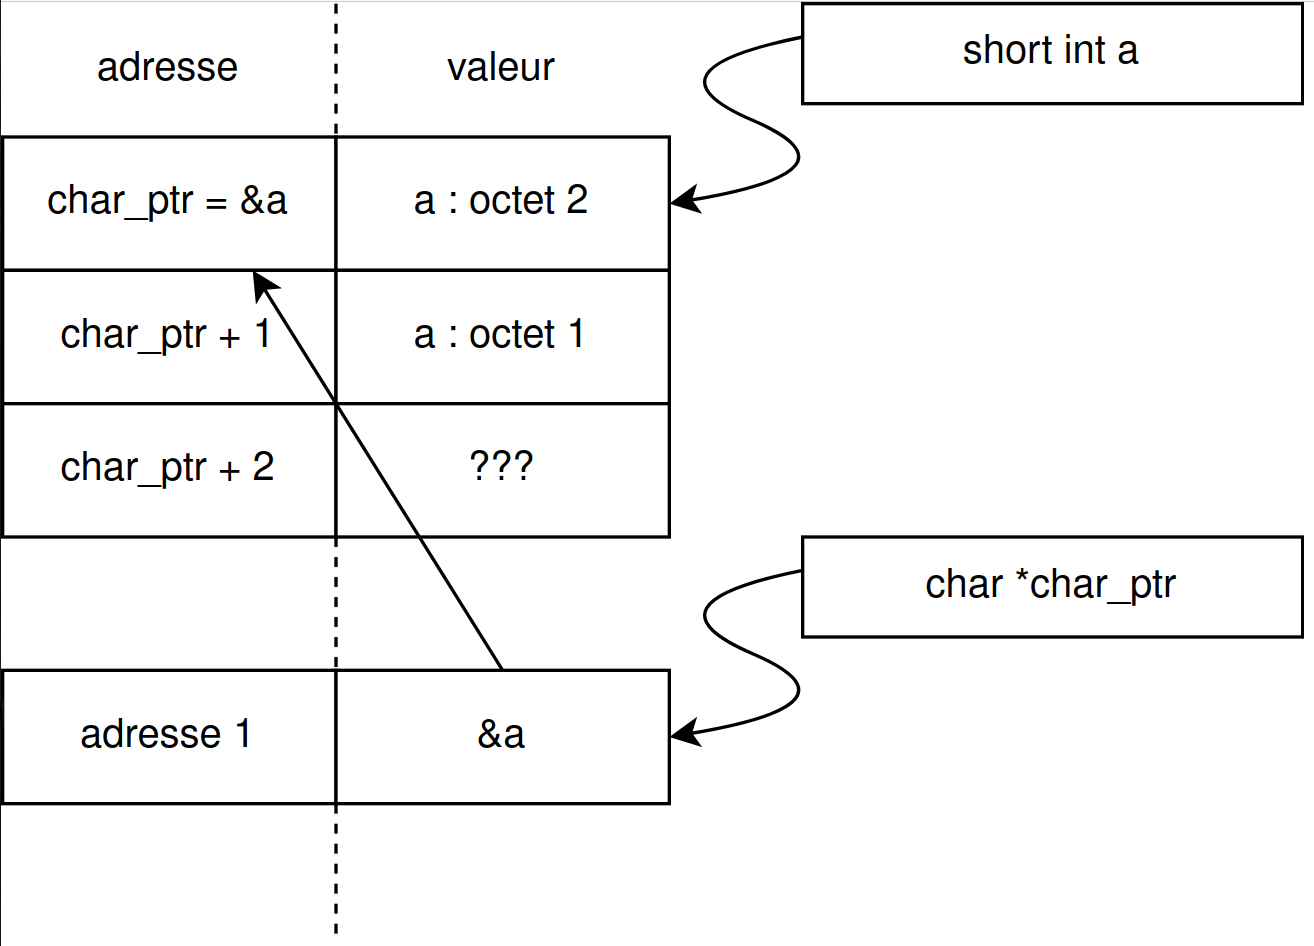
\includegraphics[width=\textwidth]{pointeur3}
	\end{center}
\end{minipage}
 
Ainsi, toutes les égalités du code suivant sont vraies :
\begin{minted}[linenos=false]{c}
char *char_ptr = char_ptr;
short int *sint_ptr = char_ptr;
int *int_ptr = char_ptr;
long int *lint_ptr = char_ptr;

// every following equality test is true :
char_ptr == sint_ptr;
char_ptr == int_ptr;
char_ptr == lint_ptr;
char_ptr + 4 ==	int_ptr + 1;
char_ptr + 2 == sint_ptr + 1;
sint_ptr + 2 == int_ptr + 1;
int_ptr + 2 == lint_ptr + 1;
\end{minted}

Toutefois, un détail reste troublant\dots l'inversion des octets 1 et 2 sur le schéma ci-dessus, que l'on observe à l'exécution du programme sur n'importe quel ordinateur possédant un UCC \textit{Intel}. 
Aucune reformulation ici, l'explication sur Wikipédia suffit : \url{https://fr.wikipedia.org/wiki/Boutisme}\footnote{Ce document n'est pas un cours d'histoire de l'informatique :`$|$}.
 
\textbf{Notation :} Avant de partir dans quelques exercices, voyons simplement une facilité d'écriture du langage C, valide pour tout pointeur \textsf{ptr} et tout entier \textsf{i} :
\begin{minted}{c}
// result of the equality test is always true :
ptr[i] == *(ptr + i);
\end{minted}
Plus un petit \textit{trick} inutile mais rigolo : comme l'addition est commutative on peut aussi écrire :
\begin{minted}{c}
// result of the equality test is always true :
(i - 1)[ptr + 1] == *(ptr + i);
\end{minted}
Les raisons de l'existence de cette facilité d'écriture seront détaillées dans la section sur les tableaux.
\subsubsection{Le pointeur quelconque : \textsf{void*}}
Un dernier cas d'utilisation du projecteur de type est celui du pointeur quelconque \textsf{void*}. En soi, un pointeur contient seulement une adresse, et il peut être intéressant dans certains programmes (voir la section sur les tableaux dynamiques) de ne conserver que l'adresse et d'``oublier'' le reste, c'est-à-dire le type du pointeur.
 
Le type spécial \textsf{void*} représente exactement cela : un pointeur non typé vers une adresse.
 
La projection de type sur un pointeur non typé \textsf{void*} permet de faire retrouver au pointeur un type :
\begin{minted}{c}
void *pointeur_quelconque = NULL;

// explicit static casting to avoid warnings at compile time :
int *int_ptr = (int*)pointeur_quelconque; 
\end{minted}
Par ailleurs, l'addition sur un pointeur non typé est ``classique'' :
\begin{minted}{c}
void *pointeur_quelconque = NULL;
printf("%p\n", pointeur_quelconque + 5); // prints 0x5
\end{minted}
Si pour l'instant l'utilisation de tels pointeurs peut rester assez absconse, cela s'éclairera dans le chapitre sur les concepts avancés du langage C. On trouvera déjà un premier exemple dans la section sur les tableaux dynamiques qui montre une application essentielle des pointeurs.
\subsection{Pointeurs itérés}
\begin{minipage}{\textwidth}
	\begin{center}
		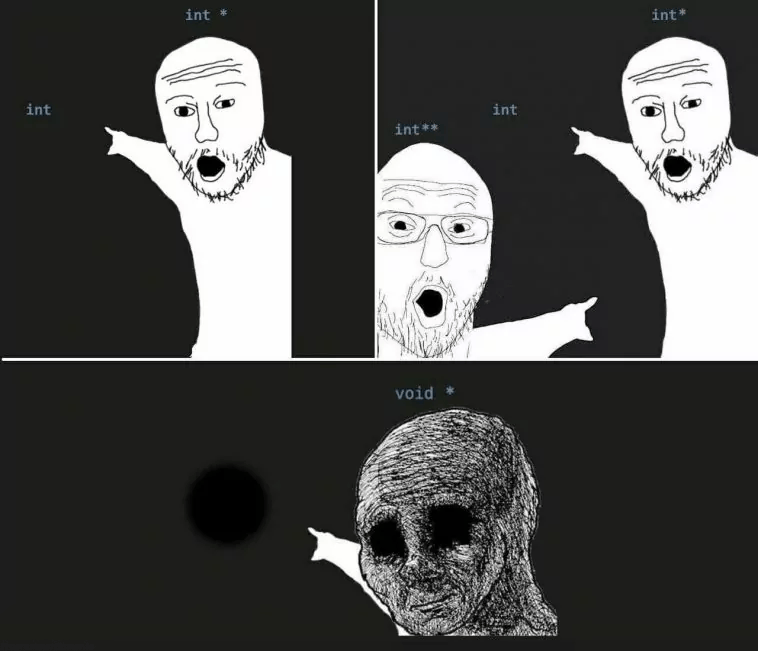
\includegraphics[width=.75\textwidth]{pointer_meme}
	\end{center}
\end{minipage}
\subsection{Exercices}
\exercise{Quelques procédures inutiles pour devenir un bot efficace} Programmer en C les procédures suivantes, et les tester sur quelques valeurs :
\begin{itemize}
	\item \textsf{void mov(int *x, int val);} : assigne à la variable pointé par $x$ la valeur $val$
	\item \textsf{void add(int *a, int *b);} : assigne à la variable pointée par $a$ la somme des valeurs des variables pointées par $a$ et $b$
	\item \textsf{void mul(int *y, int *z);} : assigne à la variable pointée par $y$ le produit des valeurs des variables pointées par $y$ et $z$
	\item \textsf{void pow(int *x, int n);} : assigne à la variable pointée par $x$ la valeur de la variable pointé par $x$ à la puissance $n$
\end{itemize}
\exercise{Interversion sans effet de bord (3)} Écrire une procédure \textsf{void swap(int *a, int *b);} qui échange les valeurs des variables pointés par $a$ et $b$ sans utiliser de variable temporaire. Quel est le comportement du programme si $x = y$ ? (c'est-à-dire que la même adresse est passé en argument pour les deux paramètres) \newline
Si cela induit une erreur de comportement de la procédure, corriger cette erreur.
 
\exercise{Distance de Manhattan}
\begin{enumerate}
	\item Écrire une fonction \textsf{double coords\_to\_point(float x, float y);} qui stocke les coordonnées d'un point dans une seule variable de type \textsf{double} à l'aide d'une projection de type.
	\item Écrire une fonction \textsf{double substract(double pA, double pB);} qui à deux points $p_{A} = (x_{A}, y_{A})$ et $p_{B} = (x_{B}, y_{B})$ renvoie : $$p_{A} - p_{B} = (x_{A} - x_{B}, y_{A} - y_{B})$$
	\item Écrire une fonction \textsf{float norme1(double p)} qui calcule la norme 1 d'un point $p = (x, y)$ :
	$$\lVert{\vec{p}}\rVert = |x| + |y|$$
	\item En déduire une fonction \textsf{float distance(double pA, double pB);} qui renvoie la distance entre deux points $p_{A}$ et $p_{B}$ associée à la norme 1. Cette distance est appelée \textit{distance de Manhattan}\footnote{Souvent utilisée en informatique du fait de sa vitesse d'exécution.}
\end{enumerate}
\textbf{Remarque : }On pourra éviter les avertissements à la compilation en effectuant des projections de type explicites.
\end{document}